 \documentclass{article}
\usepackage[utf8]{inputenc}
\usepackage[a4paper, total={7in, 10in}]{geometry}
\usepackage{braket}
\usepackage{xcolor}
\usepackage{amsmath}
\usepackage{amssymb}
\usepackage{amsfonts}
\usepackage{graphicx}
\usepackage{svg}
\usepackage{float}
\usepackage{tikz}
\usepackage[ruled,vlined]{algorithm2e}
\usepackage{multicol}
\usepackage[backend=biber,style=alphabetic,sorting=ynt]{biblatex}
\usepackage{xcolor}
%\addbibresource{sample.bib} %Import the bibliography file

\newcommand{\commentt}[1]{\textcolor{blue}{ \textbf{[COMMENT]} #1}}
\newcommand{\ctt}[1]{\commentt{#1}}
\newcommand{\prb}[1]{ \mathbf{Pr} \left[ {#1} \right]}
\newcommand{\onotation}[1]{\(\mathcal{O} \left( {#1}  \right) \)}
\newcommand{\ona}[1]{\onotation{#1}}
\newcommand{\PSI}{{\ket{\psi}}}
\newcommand{\LESn}{\ket{\psi_n}}
\newcommand{\LESa}{\ket{\phi_n}}
\newcommand{\LESs}{\frac{1}{\sqrt{n}}\sum_{i}{\ket{\left(0^{i}10^{n-i}\right)^{n}}}}
\newcommand{\Hn}{\mathcal{H}_{n}}
\newcommand{\Ep}{\frac{1}{\sqrt{2^n}}\sum^{2^n}_{x}{ \ket{xx}}}
\newcommand{\HON}{\ket{\psi_{\text{honest}}}}
\newcommand{\Lemma}{\paragraph{Lemma.}}


\setlength{\columnsep}{0.6cm}

\newcommand{\Gz}{ G_{z}^{\delta} } 

\begin{document}

\title{Quantum LTC With Positive Rate}
\author{David Ponarovsky}
\maketitle
%\begin{multicols*}{2}
\newcommand{ \Hw }{ \delta\Delta -\Delta^{\frac{1}{2}-\varepsilon}/\delta  }
	\newcommand{ \Nw }{ \Delta^{\frac{3}{2}-\varepsilon}} 
	  \newcommand{ \Gu } { \Gamma^{\cup} }
	  \newcommand{ \Guq } { \Gamma^{\cup, \square} }

    	\newcommand{ \Gsa } {\Gamma_{\square_{1}} }
	\newcommand{ \Gsb } {\Gamma_{\square_{2}} }
        \newcommand{ \Aa } { C_{A_{1}}}  
	\newcommand{ \Ab } { C_{A_{2}}}
	\newcommand{ \Ac } { C_{A_{3}}}
	\newcommand{ \Aab } { \Aa \otimes \Ab } 
	\newcommand{ \Aac } { \Aa \otimes \Ac }
	\newcommand{ \Aabc } { \Aa \otimes \Ab \otimes \Ac }
	\newcommand{ \Aabp } { \Aa^{\perp} \otimes \Ab^{\perp} } 
	\newcommand{ \Aacp } { \Aa^{\perp} \otimes \Ac^{\perp} }
	\newcommand{ \Aabcp } { \Aa^{\perp} \otimes \Ab^{\perp} \otimes \Ac^{\perp} }
	\newcommand{ \Aabpp } { \left( \Aabp \right)^\perp } 
	\newcommand{ \Aacpp } { \left( \Aacp \right)^\perp }
	\newcommand{ \Aabcpp } { \left( \Aabcp \right)^\perp }
	\newcommand{ \YY } {  y_{1}y_{2}^{\top} }
	\newcommand{ \ZZ } {  z_{1}z_{2}^{\top} } 
	\newcommand{ \TT } { \tilde{\tau} } 


  \paragraph{preamble.} preamble.  
  \begin{figure}[H]
            %\label{fig:square}
            \begin{center}
            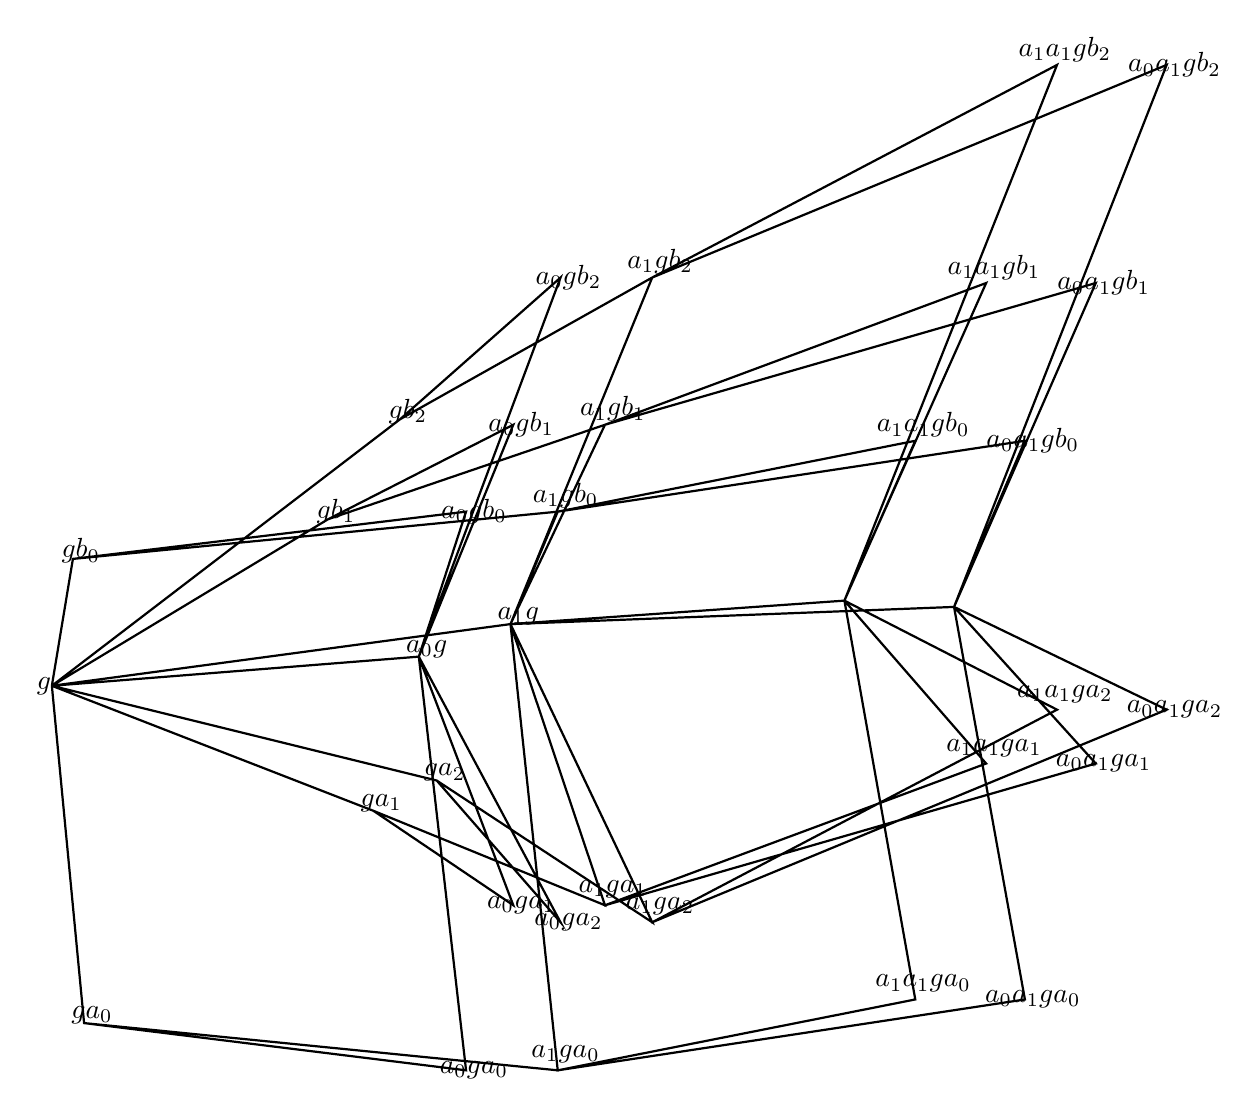
\begin{tikzpicture}
            \draw[thick](0,0)(0, 0) -- (0.26701496725008933,1.61129272670341) -- (5.260154143861819,2.21129272670341) -- (4.66015414386182,0.36986859008823236) -- (0, 0)
(0, 0) -- (3.5076976880198965,2.114975563949012) -- (5.86015414386182,3.3149755639490124) -- (4.66015414386182,0.36986859008823236) -- (0, 0)
(0, 0) -- (4.421879766371856,3.384616135560371) -- (6.4601541438618195,5.184616135560371) -- (4.66015414386182,0.36986859008823236) -- (0, 0)
(0, 0) -- (0.26701496725008933,1.61129272670341) -- (6.424350552485932,2.21129272670341) -- (5.8243505524859325,0.7833471372225075) -- (0, 0)
(0, 0) -- (3.5076976880198965,2.114975563949012) -- (7.024350552485933,3.3149755639490124) -- (5.8243505524859325,0.7833471372225075) -- (0, 0)
(0, 0) -- (4.421879766371856,3.384616135560371) -- (7.624350552485932,5.184616135560371) -- (5.8243505524859325,0.7833471372225075) -- (0, 0)
(0, 0) -- (0.4092171803757316,-4.28370953545937) -- (5.260154143861819,-4.88370953545937) -- (4.66015414386182,0.36986859008823236) -- (0, 0)
(0, 0) -- (4.08301643294336,-1.58746032994068) -- (5.86015414386182,-2.78746032994068) -- (4.66015414386182,0.36986859008823236) -- (0, 0)
(0, 0) -- (4.887626279403229,-1.2033960258055796) -- (6.4601541438618195,-3.0033960258055794) -- (4.66015414386182,0.36986859008823236) -- (0, 0)
(0, 0) -- (0.4092171803757316,-4.28370953545937) -- (6.424350552485932,-4.88370953545937) -- (5.8243505524859325,0.7833471372225075) -- (0, 0)
(0, 0) -- (4.08301643294336,-1.58746032994068) -- (7.024350552485933,-2.78746032994068) -- (5.8243505524859325,0.7833471372225075) -- (0, 0)
(0, 0) -- (4.887626279403229,-1.2033960258055796) -- (7.624350552485932,-3.0033960258055794) -- (5.8243505524859325,0.7833471372225075) -- (0, 0)
(5.8243505524859325, 0.7833471372225075) -- (6.424350552485932,2.21129272670341) -- (12.357521382004572,3.11129272670341) -- (11.457521382004572,1.0014290727299502) -- (5.8243505524859325, 0.7833471372225075)
(5.8243505524859325, 0.7833471372225075) -- (7.024350552485933,3.3149755639490124) -- (13.257521382004573,5.114975563949012) -- (11.457521382004572,1.0014290727299502) -- (5.8243505524859325, 0.7833471372225075)
(5.8243505524859325, 0.7833471372225075) -- (7.624350552485932,5.184616135560371) -- (14.157521382004571,7.884616135560371) -- (11.457521382004572,1.0014290727299502) -- (5.8243505524859325, 0.7833471372225075)
(5.8243505524859325, 0.7833471372225075) -- (6.424350552485932,2.21129272670341) -- (10.965263211254666,3.11129272670341) -- (10.065263211254665,1.081215195143528) -- (5.8243505524859325, 0.7833471372225075)
(5.8243505524859325, 0.7833471372225075) -- (7.024350552485933,3.3149755639490124) -- (11.865263211254666,5.114975563949012) -- (10.065263211254665,1.081215195143528) -- (5.8243505524859325, 0.7833471372225075)
(5.8243505524859325, 0.7833471372225075) -- (7.624350552485932,5.184616135560371) -- (12.765263211254666,7.884616135560371) -- (10.065263211254665,1.081215195143528) -- (5.8243505524859325, 0.7833471372225075)
(5.8243505524859325, 0.7833471372225075) -- (6.424350552485932,-4.88370953545937) -- (12.357521382004572,-3.98370953545937) -- (11.457521382004572,1.0014290727299502) -- (5.8243505524859325, 0.7833471372225075)
(5.8243505524859325, 0.7833471372225075) -- (7.024350552485933,-2.78746032994068) -- (13.257521382004573,-0.9874603299406799) -- (11.457521382004572,1.0014290727299502) -- (5.8243505524859325, 0.7833471372225075)
(5.8243505524859325, 0.7833471372225075) -- (7.624350552485932,-3.0033960258055794) -- (14.157521382004571,-0.30339602580557923) -- (11.457521382004572,1.0014290727299502) -- (5.8243505524859325, 0.7833471372225075)
(5.8243505524859325, 0.7833471372225075) -- (6.424350552485932,-4.88370953545937) -- (10.965263211254666,-3.98370953545937) -- (10.065263211254665,1.081215195143528) -- (5.8243505524859325, 0.7833471372225075)
(5.8243505524859325, 0.7833471372225075) -- (7.024350552485933,-2.78746032994068) -- (11.865263211254666,-0.9874603299406799) -- (10.065263211254665,1.081215195143528) -- (5.8243505524859325, 0.7833471372225075)
(5.8243505524859325, 0.7833471372225075) -- (7.624350552485932,-3.0033960258055794) -- (12.765263211254666,-0.30339602580557923) -- (10.065263211254665,1.081215195143528) -- (5.8243505524859325, 0.7833471372225075)
;
\node at (5.360154143861819,2.21129272670341) {$ a_{ 0  } gb_{ 0 } $};
\node at (5.9601541438618195,3.3149755639490124) {$ a_{ 0  } gb_{ 1 } $};
\node at (6.560154143861819,5.184616135560371) {$ a_{ 0  } gb_{ 2 } $};
\node at (6.524350552485932,2.4112927267034103) {$ a_{ 1  } gb_{ 0 } $};
\node at (7.124350552485932,3.5149755639490126) {$ a_{ 1  } gb_{ 1 } $};
\node at (7.724350552485932,5.384616135560371) {$ a_{ 1  } gb_{ 2 } $};
\node at (5.360154143861819,-4.88370953545937) {$ a_{ 0  } ga_{ 0 } $};
\node at (5.9601541438618195,-2.78746032994068) {$ a_{ 0  } ga_{ 1 } $};
\node at (6.560154143861819,-3.0033960258055794) {$ a_{ 0  } ga_{ 2 } $};
\node at (6.524350552485932,-4.68370953545937) {$ a_{ 1  } ga_{ 0 } $};
\node at (7.124350552485932,-2.5874603299406798) {$ a_{ 1  } ga_{ 1 } $};
\node at (7.724350552485932,-2.8033960258055792) {$ a_{ 1  } ga_{ 2 } $};
\node at (12.457521382004572,3.11129272670341) {$ a_{ 0  } a_{ 1 }gb_{ 0 } $};
\node at (13.357521382004572,5.114975563949012) {$ a_{ 0  } a_{ 1 }gb_{ 1 } $};
\node at (14.25752138200457,7.884616135560371) {$ a_{ 0  } a_{ 1 }gb_{ 2 } $};
\node at (11.065263211254665,3.3112927267034102) {$ a_{ 1  } a_{ 1 }gb_{ 0 } $};
\node at (11.965263211254666,5.314975563949012) {$ a_{ 1  } a_{ 1 }gb_{ 1 } $};
\node at (12.865263211254666,8.08461613556037) {$ a_{ 1  } a_{ 1 }gb_{ 2 } $};
\node at (12.457521382004572,-3.98370953545937) {$ a_{ 0  } a_{ 1 }ga_{ 0 } $};
\node at (13.357521382004572,-0.9874603299406799) {$ a_{ 0  } a_{ 1 }ga_{ 1 } $};
\node at (14.25752138200457,-0.30339602580557923) {$ a_{ 0  } a_{ 1 }ga_{ 2 } $};
\node at (11.065263211254665,-3.7837095354593697) {$ a_{ 1  } a_{ 1 }ga_{ 0 } $};
\node at (11.965263211254666,-0.7874603299406799) {$ a_{ 1  } a_{ 1 }ga_{ 1 } $};
\node at (12.865263211254666,-0.10339602580557922) {$ a_{ 1  } a_{ 1 }ga_{ 2 } $};
\node at (-0.1,0) {$ g $};
\node at (4.760154143861819,0.46986859008823234) {$ a_{ 0 }g $};
\node at (5.924350552485932,0.8833471372225075) {$ a_{ 1 }g $};
\node at (0.3670149672500893,1.7112927267034101) {$ gb_{ 0 } $};
\node at (3.6076976880198965,2.2149755639490123) {$ gb_{ 1 } $};
\node at (4.521879766371856,3.4846161355603713) {$ gb_{ 2 } $};
\node at (0.5092171803757316,-4.1837095354593705) {$ ga_{ 0 } $};
\node at (4.18301643294336,-1.48746032994068) {$ ga_{ 1 } $};
\node at (4.987626279403228,-1.1033960258055795) {$ ga_{ 2 } $};

            \end{tikzpicture}
            \end{center}
            \caption{Square of the complex, with edges $(g,ag), (agb, gb) \in E_A,
            (g,gb), (agb, ag) \in E_B.$ \label{fig:square}
            }
            \end{figure}
 \begin{figure}[H]
            %\label{fig:square}
            \begin{center}
            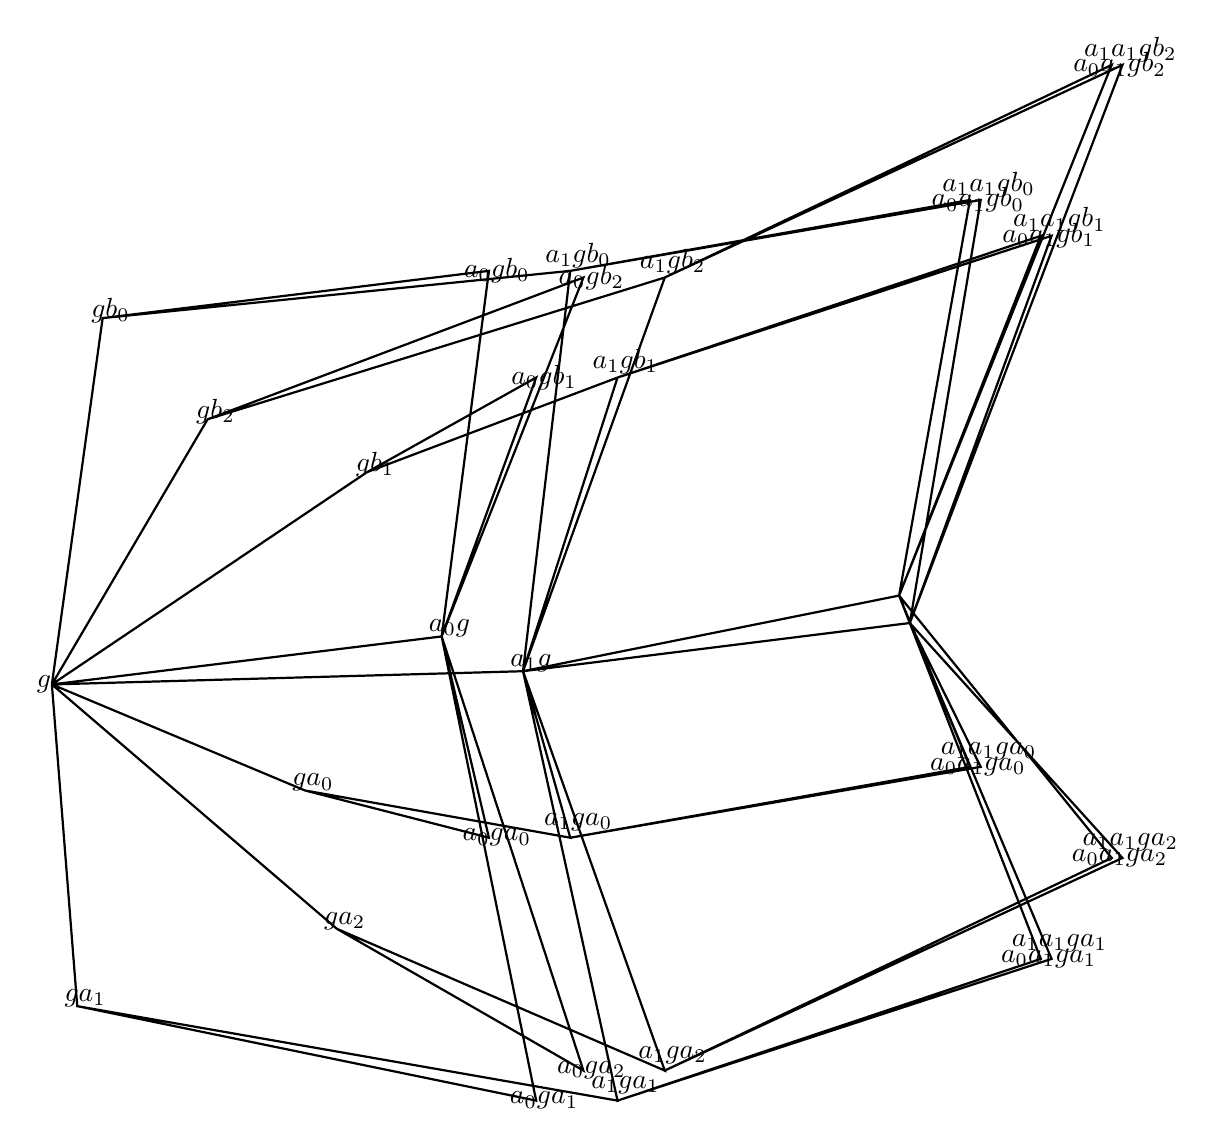
\begin{tikzpicture}
            \draw[thick](0,0)(0, 0) -- (0.6448448339309593,4.652258727715732) -- (5.550497846954821,5.2522587277157315) -- (4.950497846954821,0.609385419682218) -- (0, 0)
(0, 0) -- (4.005429215169981,2.6972151026608353) -- (6.1504978469548215,3.8972151026608355) -- (4.950497846954821,0.609385419682218) -- (0, 0)
(0, 0) -- (1.9779749413936116,3.3673886612048896) -- (6.750497846954821,5.167388661204889) -- (4.950497846954821,0.609385419682218) -- (0, 0)
(0, 0) -- (0.6448448339309593,4.652258727715732) -- (6.583732858613963,5.2522587277157315) -- (5.983732858613964,0.16776792829824982) -- (0, 0)
(0, 0) -- (4.005429215169981,2.6972151026608353) -- (7.183732858613964,3.8972151026608355) -- (5.983732858613964,0.16776792829824982) -- (0, 0)
(0, 0) -- (1.9779749413936116,3.3673886612048896) -- (7.783732858613964,5.167388661204889) -- (5.983732858613964,0.16776792829824982) -- (0, 0)
(0, 0) -- (3.214843054996499,-1.3468170581683905) -- (5.550497846954821,-1.9468170581683903) -- (4.950497846954821,0.609385419682218) -- (0, 0)
(0, 0) -- (0.3224451130646244,-4.085618690051618) -- (6.1504978469548215,-5.285618690051618) -- (4.950497846954821,0.609385419682218) -- (0, 0)
(0, 0) -- (3.6199326178578732,-3.103829090584725) -- (6.750497846954821,-4.903829090584725) -- (4.950497846954821,0.609385419682218) -- (0, 0)
(0, 0) -- (3.214843054996499,-1.3468170581683905) -- (6.583732858613963,-1.9468170581683903) -- (5.983732858613964,0.16776792829824982) -- (0, 0)
(0, 0) -- (0.3224451130646244,-4.085618690051618) -- (7.183732858613964,-5.285618690051618) -- (5.983732858613964,0.16776792829824982) -- (0, 0)
(0, 0) -- (3.6199326178578732,-3.103829090584725) -- (7.783732858613964,-4.903829090584725) -- (5.983732858613964,0.16776792829824982) -- (0, 0)
(5.983732858613964, 0.16776792829824982) -- (6.583732858613963,5.2522587277157315) -- (11.659494194294192,6.152258727715732) -- (10.759494194294192,1.1282601934965242) -- (5.983732858613964, 0.16776792829824982)
(5.983732858613964, 0.16776792829824982) -- (7.183732858613964,3.8972151026608355) -- (12.559494194294192,5.697215102660835) -- (10.759494194294192,1.1282601934965242) -- (5.983732858613964, 0.16776792829824982)
(5.983732858613964, 0.16776792829824982) -- (7.783732858613964,5.167388661204889) -- (13.45949419429419,7.867388661204889) -- (10.759494194294192,1.1282601934965242) -- (5.983732858613964, 0.16776792829824982)
(5.983732858613964, 0.16776792829824982) -- (6.583732858613963,5.2522587277157315) -- (11.796052569886035,6.152258727715732) -- (10.896052569886034,0.7800428456576101) -- (5.983732858613964, 0.16776792829824982)
(5.983732858613964, 0.16776792829824982) -- (7.183732858613964,3.8972151026608355) -- (12.696052569886035,5.697215102660835) -- (10.896052569886034,0.7800428456576101) -- (5.983732858613964, 0.16776792829824982)
(5.983732858613964, 0.16776792829824982) -- (7.783732858613964,5.167388661204889) -- (13.596052569886034,7.867388661204889) -- (10.896052569886034,0.7800428456576101) -- (5.983732858613964, 0.16776792829824982)
(5.983732858613964, 0.16776792829824982) -- (6.583732858613963,-1.9468170581683903) -- (11.659494194294192,-1.0468170581683904) -- (10.759494194294192,1.1282601934965242) -- (5.983732858613964, 0.16776792829824982)
(5.983732858613964, 0.16776792829824982) -- (7.183732858613964,-5.285618690051618) -- (12.559494194294192,-3.485618690051618) -- (10.759494194294192,1.1282601934965242) -- (5.983732858613964, 0.16776792829824982)
(5.983732858613964, 0.16776792829824982) -- (7.783732858613964,-4.903829090584725) -- (13.45949419429419,-2.2038290905847244) -- (10.759494194294192,1.1282601934965242) -- (5.983732858613964, 0.16776792829824982)
(5.983732858613964, 0.16776792829824982) -- (6.583732858613963,-1.9468170581683903) -- (11.796052569886035,-1.0468170581683904) -- (10.896052569886034,0.7800428456576101) -- (5.983732858613964, 0.16776792829824982)
(5.983732858613964, 0.16776792829824982) -- (7.183732858613964,-5.285618690051618) -- (12.696052569886035,-3.485618690051618) -- (10.896052569886034,0.7800428456576101) -- (5.983732858613964, 0.16776792829824982)
(5.983732858613964, 0.16776792829824982) -- (7.783732858613964,-4.903829090584725) -- (13.596052569886034,-2.2038290905847244) -- (10.896052569886034,0.7800428456576101) -- (5.983732858613964, 0.16776792829824982)
;
\node at (5.650497846954821,5.2522587277157315) {$ a_{ 0  } gb_{ 0 } $};
\node at (6.250497846954821,3.8972151026608355) {$ a_{ 0  } gb_{ 1 } $};
\node at (6.850497846954821,5.167388661204889) {$ a_{ 0  } gb_{ 2 } $};
\node at (6.683732858613963,5.452258727715732) {$ a_{ 1  } gb_{ 0 } $};
\node at (7.283732858613964,4.097215102660836) {$ a_{ 1  } gb_{ 1 } $};
\node at (7.883732858613963,5.367388661204889) {$ a_{ 1  } gb_{ 2 } $};
\node at (5.650497846954821,-1.9468170581683903) {$ a_{ 0  } ga_{ 0 } $};
\node at (6.250497846954821,-5.285618690051618) {$ a_{ 0  } ga_{ 1 } $};
\node at (6.850497846954821,-4.903829090584725) {$ a_{ 0  } ga_{ 2 } $};
\node at (6.683732858613963,-1.7468170581683904) {$ a_{ 1  } ga_{ 0 } $};
\node at (7.283732858613964,-5.085618690051618) {$ a_{ 1  } ga_{ 1 } $};
\node at (7.883732858613963,-4.703829090584724) {$ a_{ 1  } ga_{ 2 } $};
\node at (11.759494194294192,6.152258727715732) {$ a_{ 0  } a_{ 1 }gb_{ 0 } $};
\node at (12.659494194294192,5.697215102660835) {$ a_{ 0  } a_{ 1 }gb_{ 1 } $};
\node at (13.55949419429419,7.867388661204889) {$ a_{ 0  } a_{ 1 }gb_{ 2 } $};
\node at (11.896052569886034,6.352258727715732) {$ a_{ 1  } a_{ 1 }gb_{ 0 } $};
\node at (12.796052569886035,5.8972151026608355) {$ a_{ 1  } a_{ 1 }gb_{ 1 } $};
\node at (13.696052569886033,8.06738866120489) {$ a_{ 1  } a_{ 1 }gb_{ 2 } $};
\node at (11.759494194294192,-1.0468170581683904) {$ a_{ 0  } a_{ 1 }ga_{ 0 } $};
\node at (12.659494194294192,-3.485618690051618) {$ a_{ 0  } a_{ 1 }ga_{ 1 } $};
\node at (13.55949419429419,-2.2038290905847244) {$ a_{ 0  } a_{ 1 }ga_{ 2 } $};
\node at (11.896052569886034,-0.8468170581683905) {$ a_{ 1  } a_{ 1 }ga_{ 0 } $};
\node at (12.796052569886035,-3.285618690051618) {$ a_{ 1  } a_{ 1 }ga_{ 1 } $};
\node at (13.696052569886033,-2.0038290905847242) {$ a_{ 1  } a_{ 1 }ga_{ 2 } $};
\node at (-0.1,0) {$ g $};
\node at (5.050497846954821,0.709385419682218) {$ a_{ 0 }g $};
\node at (6.083732858613963,0.2677679282982498) {$ a_{ 1 }g $};
\node at (0.7448448339309592,4.7522587277157315) {$ gb_{ 0 } $};
\node at (4.1054292151699805,2.7972151026608354) {$ gb_{ 1 } $};
\node at (2.0779749413936117,3.4673886612048896) {$ gb_{ 2 } $};
\node at (3.314843054996499,-1.2468170581683904) {$ ga_{ 0 } $};
\node at (0.4224451130646244,-3.9856186900516177) {$ ga_{ 1 } $};
\node at (3.7199326178578733,-3.0038290905847247) {$ ga_{ 2 } $};

            \end{tikzpicture}
            \end{center}
            \caption{Square of the complex, with edges $(g,ag), (agb, gb) \in E_A,
            (g,gb), (agb, ag) \in E_B.$ \label{fig:square}
            }
            \end{figure}
 \begin{figure}[H]
            %\label{fig:square}
            \begin{center}
            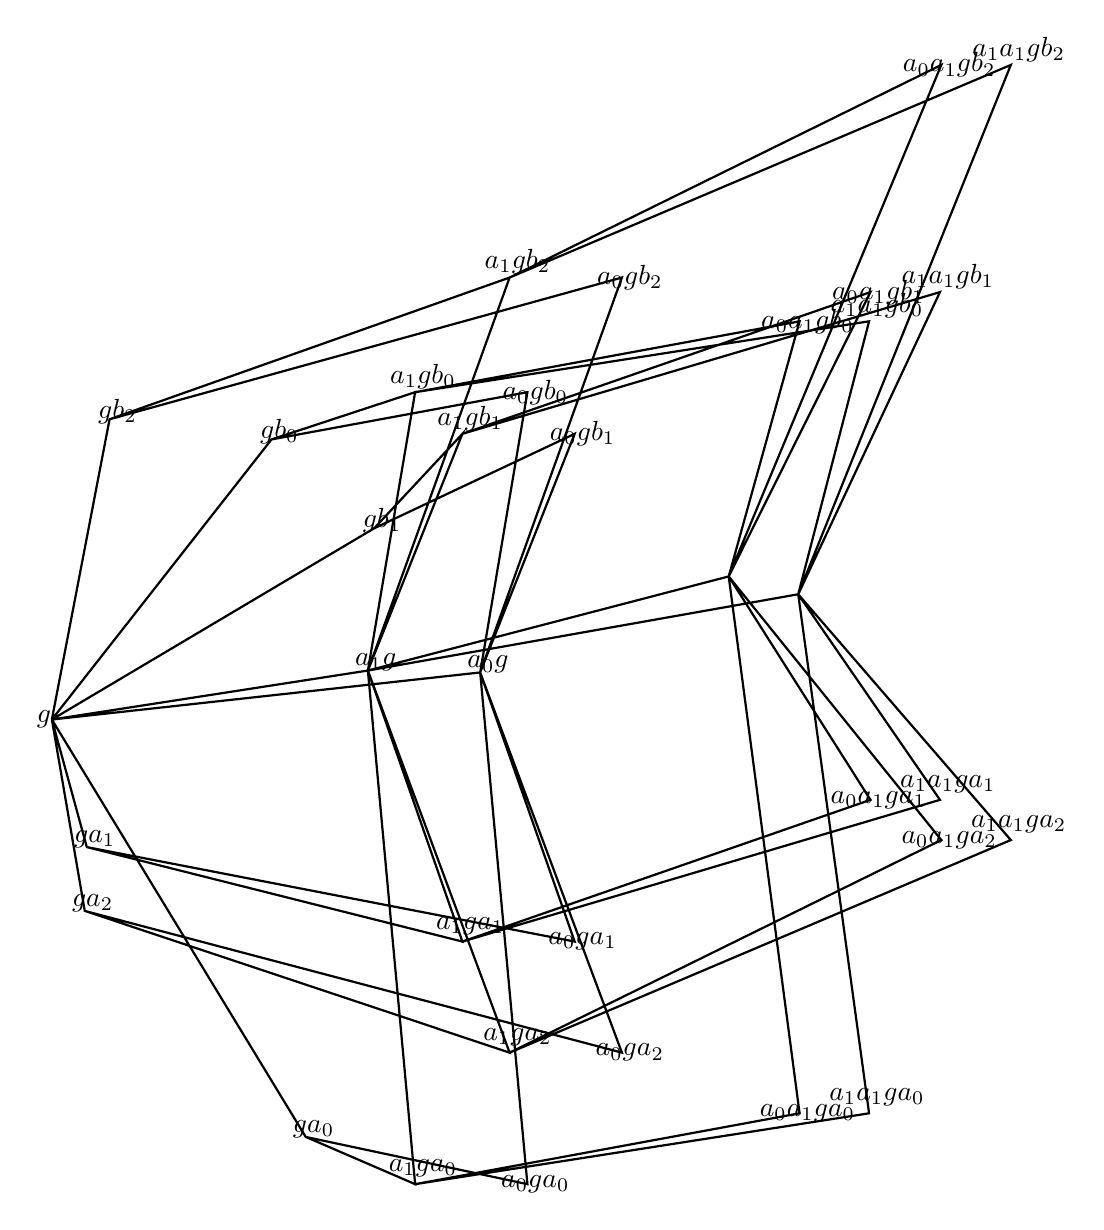
\begin{tikzpicture}
            \draw[thick](0,0)(0, 0) -- (2.7893201272767305,3.557335520202498) -- (6.0394304421008895,4.157335520202498) -- (5.43943044210089,0.5979687509182984) -- (0, 0)
(0, 0) -- (4.092881335503673,2.4283618897487105) -- (6.63943044210089,3.62836188974871) -- (5.43943044210089,0.5979687509182984) -- (0, 0)
(0, 0) -- (0.7329037591718918,3.813435725438771) -- (7.23943044210089,5.613435725438771) -- (5.43943044210089,0.5979687509182984) -- (0, 0)
(0, 0) -- (2.7893201272767305,3.557335520202498) -- (4.613508833208382,4.157335520202498) -- (4.013508833208382,0.6221517527661181) -- (0, 0)
(0, 0) -- (4.092881335503673,2.4283618897487105) -- (5.213508833208382,3.62836188974871) -- (4.013508833208382,0.6221517527661181) -- (0, 0)
(0, 0) -- (0.7329037591718918,3.813435725438771) -- (5.813508833208382,5.613435725438771) -- (4.013508833208382,0.6221517527661181) -- (0, 0)
(0, 0) -- (3.2240394407112154,-5.300576369595899) -- (6.0394304421008895,-5.900576369595899) -- (5.43943044210089,0.5979687509182984) -- (0, 0)
(0, 0) -- (0.44381228097165215,-1.6197478728072525) -- (6.63943044210089,-2.8197478728072527) -- (5.43943044210089,0.5979687509182984) -- (0, 0)
(0, 0) -- (0.41768789442829135,-2.430303535367476) -- (7.23943044210089,-4.230303535367476) -- (5.43943044210089,0.5979687509182984) -- (0, 0)
(0, 0) -- (3.2240394407112154,-5.300576369595899) -- (4.613508833208382,-5.900576369595899) -- (4.013508833208382,0.6221517527661181) -- (0, 0)
(0, 0) -- (0.44381228097165215,-1.6197478728072525) -- (5.213508833208382,-2.8197478728072527) -- (4.013508833208382,0.6221517527661181) -- (0, 0)
(0, 0) -- (0.41768789442829135,-2.430303535367476) -- (5.813508833208382,-4.230303535367476) -- (4.013508833208382,0.6221517527661181) -- (0, 0)
(4.013508833208382, 0.6221517527661181) -- (4.613508833208382,4.157335520202498) -- (9.495842207560885,5.057335520202498) -- (8.595842207560885,1.8176268765986756) -- (4.013508833208382, 0.6221517527661181)
(4.013508833208382, 0.6221517527661181) -- (5.213508833208382,3.62836188974871) -- (10.395842207560886,5.42836188974871) -- (8.595842207560885,1.8176268765986756) -- (4.013508833208382, 0.6221517527661181)
(4.013508833208382, 0.6221517527661181) -- (5.813508833208382,5.613435725438771) -- (11.295842207560884,8.313435725438772) -- (8.595842207560885,1.8176268765986756) -- (4.013508833208382, 0.6221517527661181)
(4.013508833208382, 0.6221517527661181) -- (4.613508833208382,4.157335520202498) -- (10.378632255404762,5.057335520202498) -- (9.478632255404762,1.5910683902593776) -- (4.013508833208382, 0.6221517527661181)
(4.013508833208382, 0.6221517527661181) -- (5.213508833208382,3.62836188974871) -- (11.278632255404762,5.42836188974871) -- (9.478632255404762,1.5910683902593776) -- (4.013508833208382, 0.6221517527661181)
(4.013508833208382, 0.6221517527661181) -- (5.813508833208382,5.613435725438771) -- (12.17863225540476,8.313435725438772) -- (9.478632255404762,1.5910683902593776) -- (4.013508833208382, 0.6221517527661181)
(4.013508833208382, 0.6221517527661181) -- (4.613508833208382,-5.900576369595899) -- (9.495842207560885,-5.0005763695958985) -- (8.595842207560885,1.8176268765986756) -- (4.013508833208382, 0.6221517527661181)
(4.013508833208382, 0.6221517527661181) -- (5.213508833208382,-2.8197478728072527) -- (10.395842207560886,-1.0197478728072527) -- (8.595842207560885,1.8176268765986756) -- (4.013508833208382, 0.6221517527661181)
(4.013508833208382, 0.6221517527661181) -- (5.813508833208382,-4.230303535367476) -- (11.295842207560884,-1.5303035353674757) -- (8.595842207560885,1.8176268765986756) -- (4.013508833208382, 0.6221517527661181)
(4.013508833208382, 0.6221517527661181) -- (4.613508833208382,-5.900576369595899) -- (10.378632255404762,-5.0005763695958985) -- (9.478632255404762,1.5910683902593776) -- (4.013508833208382, 0.6221517527661181)
(4.013508833208382, 0.6221517527661181) -- (5.213508833208382,-2.8197478728072527) -- (11.278632255404762,-1.0197478728072527) -- (9.478632255404762,1.5910683902593776) -- (4.013508833208382, 0.6221517527661181)
(4.013508833208382, 0.6221517527661181) -- (5.813508833208382,-4.230303535367476) -- (12.17863225540476,-1.5303035353674757) -- (9.478632255404762,1.5910683902593776) -- (4.013508833208382, 0.6221517527661181)
;
\node at (6.139430442100889,4.157335520202498) {$ a_{ 0  } gb_{ 0 } $};
\node at (6.73943044210089,3.62836188974871) {$ a_{ 0  } gb_{ 1 } $};
\node at (7.339430442100889,5.613435725438771) {$ a_{ 0  } gb_{ 2 } $};
\node at (4.713508833208381,4.357335520202498) {$ a_{ 1  } gb_{ 0 } $};
\node at (5.313508833208382,3.8283618897487104) {$ a_{ 1  } gb_{ 1 } $};
\node at (5.913508833208382,5.813435725438771) {$ a_{ 1  } gb_{ 2 } $};
\node at (6.139430442100889,-5.900576369595899) {$ a_{ 0  } ga_{ 0 } $};
\node at (6.73943044210089,-2.8197478728072527) {$ a_{ 0  } ga_{ 1 } $};
\node at (7.339430442100889,-4.230303535367476) {$ a_{ 0  } ga_{ 2 } $};
\node at (4.713508833208381,-5.700576369595899) {$ a_{ 1  } ga_{ 0 } $};
\node at (5.313508833208382,-2.6197478728072525) {$ a_{ 1  } ga_{ 1 } $};
\node at (5.913508833208382,-4.030303535367476) {$ a_{ 1  } ga_{ 2 } $};
\node at (9.595842207560885,5.057335520202498) {$ a_{ 0  } a_{ 1 }gb_{ 0 } $};
\node at (10.495842207560885,5.42836188974871) {$ a_{ 0  } a_{ 1 }gb_{ 1 } $};
\node at (11.395842207560884,8.313435725438772) {$ a_{ 0  } a_{ 1 }gb_{ 2 } $};
\node at (10.478632255404762,5.257335520202498) {$ a_{ 1  } a_{ 1 }gb_{ 0 } $};
\node at (11.378632255404762,5.62836188974871) {$ a_{ 1  } a_{ 1 }gb_{ 1 } $};
\node at (12.27863225540476,8.513435725438772) {$ a_{ 1  } a_{ 1 }gb_{ 2 } $};
\node at (9.595842207560885,-5.0005763695958985) {$ a_{ 0  } a_{ 1 }ga_{ 0 } $};
\node at (10.495842207560885,-1.0197478728072527) {$ a_{ 0  } a_{ 1 }ga_{ 1 } $};
\node at (11.395842207560884,-1.5303035353674757) {$ a_{ 0  } a_{ 1 }ga_{ 2 } $};
\node at (10.478632255404762,-4.800576369595898) {$ a_{ 1  } a_{ 1 }ga_{ 0 } $};
\node at (11.378632255404762,-0.8197478728072527) {$ a_{ 1  } a_{ 1 }ga_{ 1 } $};
\node at (12.27863225540476,-1.3303035353674757) {$ a_{ 1  } a_{ 1 }ga_{ 2 } $};
\node at (-0.1,0) {$ g $};
\node at (5.5394304421008895,0.6979687509182984) {$ a_{ 0 }g $};
\node at (4.113508833208382,0.7221517527661181) {$ a_{ 1 }g $};
\node at (2.8893201272767306,3.657335520202498) {$ gb_{ 0 } $};
\node at (4.192881335503673,2.5283618897487106) {$ gb_{ 1 } $};
\node at (0.8329037591718917,3.913435725438771) {$ gb_{ 2 } $};
\node at (3.3240394407112155,-5.2005763695958995) {$ ga_{ 0 } $};
\node at (0.5438122809716521,-1.5197478728072524) {$ ga_{ 1 } $};
\node at (0.5176878944282913,-2.330303535367476) {$ ga_{ 2 } $};

            \end{tikzpicture}
            \end{center}
            \caption{Square of the complex, with edges $(g,ag), (agb, gb) \in E_A,
            (g,gb), (agb, ag) \in E_B.$ \label{fig:square}
            }
            \end{figure}
 \begin{figure}[H]
            %\label{fig:square}
            \begin{center}
            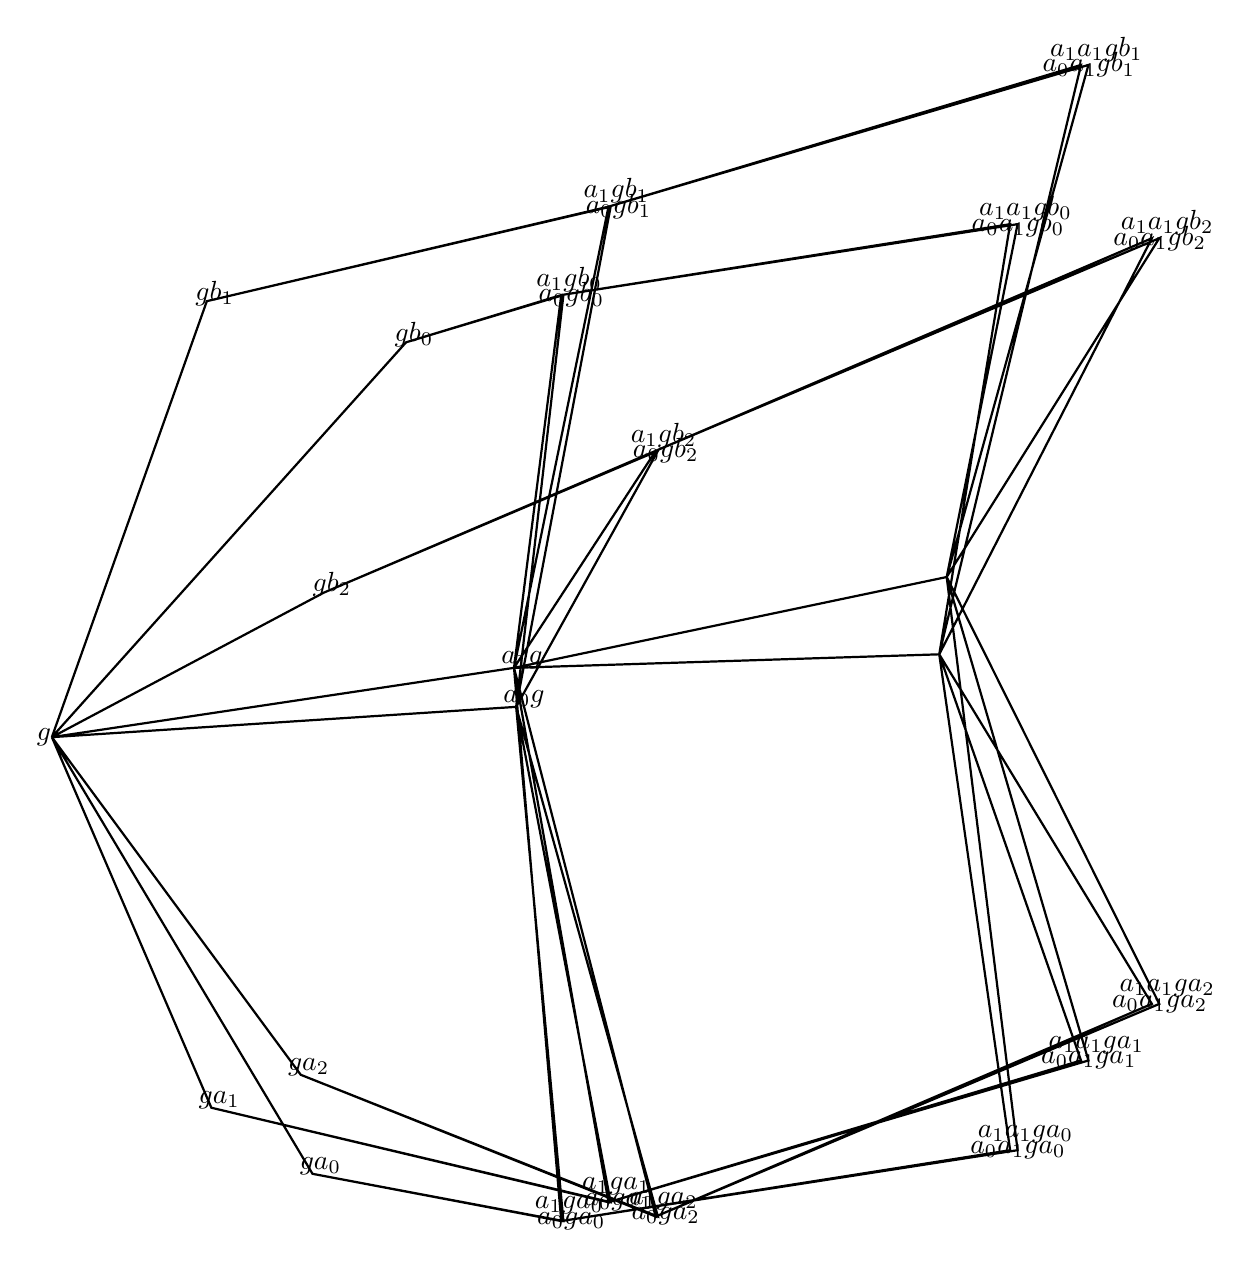
\begin{tikzpicture}
            \draw[thick](0,0)(0, 0) -- (4.498712317155559,5.014593825195722) -- (6.49645265773353,5.614593825195722) -- (5.896452657733531,0.384567514437377) -- (0, 0)
(0, 0) -- (1.9682415725458196,5.537013599262631) -- (7.096452657733531,6.737013599262631) -- (5.896452657733531,0.384567514437377) -- (0, 0)
(0, 0) -- (3.455865628480282,1.836202542513425) -- (7.696452657733531,3.636202542513425) -- (5.896452657733531,0.384567514437377) -- (0, 0)
(0, 0) -- (4.498712317155559,5.014593825195722) -- (6.469093162251695,5.614593825195722) -- (5.869093162251695,0.8800890798160514) -- (0, 0)
(0, 0) -- (1.9682415725458196,5.537013599262631) -- (7.069093162251695,6.737013599262631) -- (5.869093162251695,0.8800890798160514) -- (0, 0)
(0, 0) -- (3.455865628480282,1.836202542513425) -- (7.669093162251695,3.636202542513425) -- (5.869093162251695,0.8800890798160514) -- (0, 0)
(0, 0) -- (3.3102194845530386,-5.545616160303175) -- (6.49645265773353,-6.145616160303175) -- (5.896452657733531,0.384567514437377) -- (0, 0)
(0, 0) -- (2.0256683458695752,-4.706291281083592) -- (7.096452657733531,-5.906291281083592) -- (5.896452657733531,0.384567514437377) -- (0, 0)
(0, 0) -- (3.1607044960123627,-4.287787686350895) -- (7.696452657733531,-6.087787686350895) -- (5.896452657733531,0.384567514437377) -- (0, 0)
(0, 0) -- (3.3102194845530386,-5.545616160303175) -- (6.469093162251695,-6.145616160303175) -- (5.869093162251695,0.8800890798160514) -- (0, 0)
(0, 0) -- (2.0256683458695752,-4.706291281083592) -- (7.069093162251695,-5.906291281083592) -- (5.869093162251695,0.8800890798160514) -- (0, 0)
(0, 0) -- (3.1607044960123627,-4.287787686350895) -- (7.669093162251695,-6.087787686350895) -- (5.869093162251695,0.8800890798160514) -- (0, 0)
(5.869093162251695, 0.8800890798160514) -- (6.469093162251695,5.614593825195722) -- (12.169835302806499,6.514593825195722) -- (11.269835302806499,1.0517779722844496) -- (5.869093162251695, 0.8800890798160514)
(5.869093162251695, 0.8800890798160514) -- (7.069093162251695,6.737013599262631) -- (13.0698353028065,8.53701359926263) -- (11.269835302806499,1.0517779722844496) -- (5.869093162251695, 0.8800890798160514)
(5.869093162251695, 0.8800890798160514) -- (7.669093162251695,3.636202542513425) -- (13.969835302806498,6.3362025425134245) -- (11.269835302806499,1.0517779722844496) -- (5.869093162251695, 0.8800890798160514)
(5.869093162251695, 0.8800890798160514) -- (6.469093162251695,5.614593825195722) -- (12.264232527141194,6.514593825195722) -- (11.364232527141194,2.03358610915196) -- (5.869093162251695, 0.8800890798160514)
(5.869093162251695, 0.8800890798160514) -- (7.069093162251695,6.737013599262631) -- (13.164232527141195,8.53701359926263) -- (11.364232527141194,2.03358610915196) -- (5.869093162251695, 0.8800890798160514)
(5.869093162251695, 0.8800890798160514) -- (7.669093162251695,3.636202542513425) -- (14.064232527141193,6.3362025425134245) -- (11.364232527141194,2.03358610915196) -- (5.869093162251695, 0.8800890798160514)
(5.869093162251695, 0.8800890798160514) -- (6.469093162251695,-6.145616160303175) -- (12.169835302806499,-5.245616160303174) -- (11.269835302806499,1.0517779722844496) -- (5.869093162251695, 0.8800890798160514)
(5.869093162251695, 0.8800890798160514) -- (7.069093162251695,-5.906291281083592) -- (13.0698353028065,-4.1062912810835925) -- (11.269835302806499,1.0517779722844496) -- (5.869093162251695, 0.8800890798160514)
(5.869093162251695, 0.8800890798160514) -- (7.669093162251695,-6.087787686350895) -- (13.969835302806498,-3.3877876863508947) -- (11.269835302806499,1.0517779722844496) -- (5.869093162251695, 0.8800890798160514)
(5.869093162251695, 0.8800890798160514) -- (6.469093162251695,-6.145616160303175) -- (12.264232527141194,-5.245616160303174) -- (11.364232527141194,2.03358610915196) -- (5.869093162251695, 0.8800890798160514)
(5.869093162251695, 0.8800890798160514) -- (7.069093162251695,-5.906291281083592) -- (13.164232527141195,-4.1062912810835925) -- (11.364232527141194,2.03358610915196) -- (5.869093162251695, 0.8800890798160514)
(5.869093162251695, 0.8800890798160514) -- (7.669093162251695,-6.087787686350895) -- (14.064232527141193,-3.3877876863508947) -- (11.364232527141194,2.03358610915196) -- (5.869093162251695, 0.8800890798160514)
;
\node at (6.59645265773353,5.614593825195722) {$ a_{ 0  } gb_{ 0 } $};
\node at (7.196452657733531,6.737013599262631) {$ a_{ 0  } gb_{ 1 } $};
\node at (7.79645265773353,3.636202542513425) {$ a_{ 0  } gb_{ 2 } $};
\node at (6.569093162251694,5.814593825195722) {$ a_{ 1  } gb_{ 0 } $};
\node at (7.169093162251695,6.937013599262631) {$ a_{ 1  } gb_{ 1 } $};
\node at (7.7690931622516946,3.836202542513425) {$ a_{ 1  } gb_{ 2 } $};
\node at (6.59645265773353,-6.145616160303175) {$ a_{ 0  } ga_{ 0 } $};
\node at (7.196452657733531,-5.906291281083592) {$ a_{ 0  } ga_{ 1 } $};
\node at (7.79645265773353,-6.087787686350895) {$ a_{ 0  } ga_{ 2 } $};
\node at (6.569093162251694,-5.9456161603031745) {$ a_{ 1  } ga_{ 0 } $};
\node at (7.169093162251695,-5.706291281083592) {$ a_{ 1  } ga_{ 1 } $};
\node at (7.7690931622516946,-5.887787686350895) {$ a_{ 1  } ga_{ 2 } $};
\node at (12.269835302806499,6.514593825195722) {$ a_{ 0  } a_{ 1 }gb_{ 0 } $};
\node at (13.169835302806499,8.53701359926263) {$ a_{ 0  } a_{ 1 }gb_{ 1 } $};
\node at (14.069835302806498,6.3362025425134245) {$ a_{ 0  } a_{ 1 }gb_{ 2 } $};
\node at (12.364232527141194,6.714593825195722) {$ a_{ 1  } a_{ 1 }gb_{ 0 } $};
\node at (13.264232527141194,8.73701359926263) {$ a_{ 1  } a_{ 1 }gb_{ 1 } $};
\node at (14.164232527141193,6.536202542513425) {$ a_{ 1  } a_{ 1 }gb_{ 2 } $};
\node at (12.269835302806499,-5.245616160303174) {$ a_{ 0  } a_{ 1 }ga_{ 0 } $};
\node at (13.169835302806499,-4.1062912810835925) {$ a_{ 0  } a_{ 1 }ga_{ 1 } $};
\node at (14.069835302806498,-3.3877876863508947) {$ a_{ 0  } a_{ 1 }ga_{ 2 } $};
\node at (12.364232527141194,-5.045616160303174) {$ a_{ 1  } a_{ 1 }ga_{ 0 } $};
\node at (13.264232527141194,-3.9062912810835924) {$ a_{ 1  } a_{ 1 }ga_{ 1 } $};
\node at (14.164232527141193,-3.1877876863508945) {$ a_{ 1  } a_{ 1 }ga_{ 2 } $};
\node at (-0.1,0) {$ g $};
\node at (5.99645265773353,0.484567514437377) {$ a_{ 0 }g $};
\node at (5.969093162251695,0.9800890798160514) {$ a_{ 1 }g $};
\node at (4.598712317155559,5.114593825195722) {$ gb_{ 0 } $};
\node at (2.0682415725458196,5.63701359926263) {$ gb_{ 1 } $};
\node at (3.555865628480282,1.936202542513425) {$ gb_{ 2 } $};
\node at (3.4102194845530387,-5.445616160303175) {$ ga_{ 0 } $};
\node at (2.1256683458695753,-4.6062912810835925) {$ ga_{ 1 } $};
\node at (3.260704496012363,-4.187787686350895) {$ ga_{ 2 } $};

            \end{tikzpicture}
            \end{center}
            \caption{Square of the complex, with edges $(g,ag), (agb, gb) \in E_A,
            (g,gb), (agb, ag) \in E_B.$ \label{fig:square}
            }
            \end{figure}
 
%\end{multicols*}
  % \printbibliography 
\end{document}

 